\chapter{2020年\textsf{HDU} 概率论与数理统计期中试卷\textsf B}

\begin{minipage}{0.32\textwidth}
    \textbf{开课学院}：理学院
      
    \textbf{课程编码}：A0714040
\end{minipage}
\hfill
\begin{minipage}{0.32\textwidth}
    \textbf{解析制作}：\textsc{Ljl, Zzr, Zwx, Xxy}

    \textbf{\,\hologo{TeX}~排版}：\textsc{Mingyu Hsia}
\end{minipage}
\hfill
\begin{minipage}{0.15\textwidth}
    \centering
    \begin{tikzpicture}
        \node [inner sep=0] at (0,0) {
            \qrcode[height=3em,level=M]{https://qm.qq.com/q/OlkSiy9W04}};
        \fill [color=white,rounded corners] (-.5em,-.5em) rectangle (.5em,.5em);
        \node [inner sep=0] at (0,0) {\color{MidnightBlue}\scriptsize\faIcon{qq}};
    \end{tikzpicture}

    \scriptsize\href{https://qm.qq.com/q/OlkSiy9W04}{\itshape 未央数学营}
\end{minipage}
\hfill
\begin{minipage}{0.15\textwidth}
    \centering
    \begin{tikzpicture}
        \node [inner sep=0] at (0,0) {
            \qrcode[height=3em,level=M]{http://weixin.qq.com/r/DBIABcHEqgnWKIVmb0eI}};
        \fill [color=white,rounded corners] (-.5em,-.5em) rectangle (.5em,.5em);
        \node [inner sep=0] at (0,0) {\color{DarkGreen}\scriptsize\faIcon{weixin}};
    \end{tikzpicture}

    \scriptsize\href{http://weixin.qq.com/r/DBIABcHEqgnWKIVmb0eI}{\itshape 未央学社}
\end{minipage}

\section{选择题}

\begin{problem}
    事件$A$，$B$若满足$P(AB)=P(A)P(B)$，则$A$，$B$
    \begin{tasks}(4)
        \task[\true] 独立
        \task 不独立
        \task 互斥
        \task 不互斥
    \end{tasks}
\end{problem}
\begin{solution}
    详见概率论与数理统计课本第一章第六节.
\end{solution}

\begin{problem}
    设$f(x)$是随机变量$X$的概率密度函数，则一定成立的是
    \begin{tasks}(2)
        \task $f(x)$定义域为$[0,1]$
        \task[\true] $f(x)$非负
        \task $f(x)$的值域为$[0,1]$
        \task $f(x)$连续
    \end{tasks}
\end{problem}
\begin{solution}\leavevmode
    \begin{tasks}[label=\labelitemi](2)
        \task! 由于定义域可取$(-\infty,+\infty)$且可以间断，所以A、D选项错误.
        \task 值域为$[0,1)$，所以C选项错误.
        \task 由于概率为正值或$0$，所以B选项正确.
    \end{tasks}
\end{solution}

\begin{problem}
    若连续型随机变量$X$的分布函数为$F(x)=\begin{cases}
        0, & x<0\\
        Ax, & 0\leq x<1\\
        1, & x\geq 1
    \end{cases}$，则$A=$
    \begin{tasks}(4)
        \task $0$
        \task $\ln2$
        \task[\true] $1$
        \task $\e$
    \end{tasks}
\end{problem}
\begin{solution}
    求得$f(x)=A\ (0\leq x<1)$. 由于$\int_0^1f(x)\d x=1$，所以$A=1$.
\end{solution}

\begin{problem}
    设$X\sim N(1,3)$，要使$P(X\leq c)=1/2$，则$c$的值为
    \begin{tasks}(4)
        \task[\true] $1$
        \task $2$
        \task $3$
        \task $4$
    \end{tasks}
\end{problem}
\begin{solution}
    由于$P\ab\{\frac{x-1}{\sqrt3}\leq\frac{c-1}{\sqrt3}=\frac12\}$，所以$\Phi\ab(\frac{c-1}{\sqrt3})=\frac12$，$c=1$.
\end{solution}

\begin{problem}
    某人射击的命中率为$0.4$，用$X$表示他在3次独立射击中命中目标的次数，则$X$的分布为
    \begin{tasks}(4)
        \task $0-1$分布
        \task[\true] 二项分布
        \task 均匀分布
        \task 泊松分布
    \end{tasks}
\end{problem}
\begin{solution}
    即3次独立重复实验，服从$b(0.4,3)$的二项分布. 所以B选项正确.
\end{solution}

\section{填空题}

\begin{problem}
    设$A$、$B$为互不相容的随机事件$P(A)=0.3$，$P(B)=0.5$，则$P(A\cup B)=$\ans{$0.8$}.
\end{problem}
\begin{solution}
    $P(A\cup B)=P(A)+P(B)-P(AB)$，而$AB$互不相容，所以$P(AB)=0$，$P(A\cup B)=0.8$.
\end{solution}

\begin{problem}
    设$P(A)=0.4$，$P(B)=0.3$，$P(A\cup B)=0.6$，则$P(A\overline B)=$\ans{$0.3$}.
\end{problem}
\begin{solution}
    $P(AB)=P(A)+P(B)-P(A\cup B)=0.1$，$P(A\overline B)=P(A)-P(AB)=0.3$.
\end{solution}

\begin{problem}
    设随机变量$X$的概率密度$f_(x)=\begin{cases}
        1, & 0\leq x<1\\0, & \text{else}
    \end{cases}$，则$P\{X>0.4\}=$\ans{$0.6$}.
\end{problem}
\begin{solution}
    $P\{x>0.4\}=\int_{0.4}^{+\infty}f(x)\d x=\int_{0.4}^11\d x=0.6$.
\end{solution}

\begin{problem}
    设有10件产品，其中有4件次品，今从中任取出1件为次品的概率是\ans{$0.4$}.
\end{problem}
\begin{solution}
    $P=4/10=0.4$
\end{solution}

\begin{problem}
    设$X\sim N(0,1)$，则概率密度函数$f(x)=$\ans{$\e^{-x^2/2}/\sqrt{2\pi}$}.
\end{problem}
\begin{solution}
    对于$X\sim N(\mu,\sigma^2)$，其概率密度分布函数为$f(x)=\e^{-(x-\mu)^2/2\sigma^2}/\sqrt{2\pi}\sigma$. 所以$X\sim N(0,1)$的概率密度函数为$f(x)=\e^{-x^2/2}/\sqrt{2\pi}$.
\end{solution}

\section{计算题}

\begin{problem}
    甲、乙、丙三个同学同时独立参加考试，不及格的概率分别为：$0.2$，$0.3$，$0.4$. 求恰有两位同学不及格的概率.
\end{problem}
\solute3
\begin{solution}
    设$A$、$B$、$C$事件分别为甲乙、乙丙、甲丙不及格. 则``恰有两位同学不及格''概率为
    \[P\{A\}+P\{B\}+P\{C\}=0.2\times0.3\times(1-0.4)+0.3\times0.4\times(1-0.2)+0.2\times0.4\times(1-0.3)=0.188\]
\end{solution}

\begin{problem}
    一批产品由甲乙两厂生产，已知甲厂的产品占总产量的三分之一，且甲乙两厂 产品的次品率分别为2\%和 1\%，现随机挑选一件.
    \begin{enumerate}
        \item 求这批产品的次品率.
        \item 若取得次品，求其为甲厂生产的概率.
    \end{enumerate}
\end{problem}
\solute4
\begin{solution}\leavevmode
    \begin{enumerate}
        \item 设总量为$x$，则$\text{次品率}=\text{不合格品数量}/\text{总量}=(0.02\cdot x/3+0.01\cdot2x/3)/x=1.3\%$.
        \item $P=\text{甲厂次品数量}/\text{总次品数量}=(0.02\cdot x/3)/(0.02\cdot x/3+0.01\cdot2x/3)=50\%$.
    \end{enumerate}
\end{solution}

\begin{paracol}{2}
\begin{problem}
    离散型随机变量$X$的分布律如右图所示.
\begin{multicols}{2}
    \begin{enumerate}
        \item 求$a$的值.
        \item 求$X$的分布函数.
        \item 求$P(0<X\leq3/2)$.
    \end{enumerate}
\end{multicols}
\switchcolumn\vspace*{\fill}\centering
    \begin{tabular}{ccccc}
        \toprule
        $X$ & $-1$ & $0$ & $1$ & $2$\\
        \midrule
        $p_k$ & $0.2$ & $0.5$ & $a$ & $0.2$\\
        \bottomrule
    \end{tabular}\vspace*{\fill}
\end{problem}
\end{paracol}
\solute5
\begin{solution}\leavevmode
    \begin{multicols}{2}
        \begin{enumerate}
            \item $a=1-0.2-0.2-0.5=0.1$.
            \item 
            $F(x)=P(X\leq x)=\begin{cases}
                0 & x<-1\\
                0.2 & -1\leq x<0\\
                0.7 & 0\leq x<1\\
                0.8 & 1\leq x<2\\
                1 & 2\leq x
            \end{cases}$
            \item $P(0<x\leq3/2)=0.1$.
        \end{enumerate}
    \end{multicols}
\end{solution}

\begin{paracol}{2}
\begin{problem}
    设离散型随机变量$X$ 的分布函数为
    \[F(x)=\begin{cases}
        0 & x<-2\\
        0.4 & -2\leq x<0\\
        0.7 & 0\leq x<2\\
        1 & x\geq 2
    \end{cases}\]
    求$X$的分布律.
\end{problem}
\switchcolumn
\solute0
\begin{solution}
    对离散型分布
    \begin{table}[H]
        \centering
        \begin{tabular}{cccc}
            \toprule
            $X$  & $-2$ & $0$ & $2$\\
            \midrule
            $P$ & $0.4$ & $0.3$ & $0.3$\\
            \bottomrule
        \end{tabular}
    \end{table}
\end{solution}
\end{paracol}

\begin{problem}
    设随机变量$X$具有概率密度函数：$f(x)=\begin{cases}
        2x, & 0<x<1\\
        0,  & \text{else}
    \end{cases}$. 求$Y=X-4$的概率密度函数.
\end{problem}
\solute5
\begin{solution}\leavevmode
    \begin{itemize}
        \item $F_Y(y)=P(Y\leq y)>P\{(x-4)\leq y\}=P\{x\leq y+4\}$.
        \item 当$0<x<1$时，$-4<y<-3$. 所以当$y\leq-4$时，$F(y)=0$.
        \item 当$-4<y<-3$时，$F_Y(y)=P(Y\leq y)=P(x\leq y+4)=\int_0^{y+4}2x\d x=(y+4)^2$.
        \item 当$y\geq-3$时，$F_Y(y)=1$. 综上，$Y=X-4$的函数为
        \[f_Y(y)=F_Y'(y)=\begin{cases}
            2(y+4), & -4<y<-3\\0, & \text{else}
        \end{cases}\]
    \end{itemize}
\end{solution}

\begin{paracol}{2}
\begin{problem}
    已知二维离散型随机变量$(X,Y)$的分布律如右图所示.
    \begin{multicols}{2}
        \begin{enumerate}
            \item 求$X$的边缘分布律.
            \item 求$X+Y$的分布律.
            \item 求$P\{X+Y\leq1\}$.
            \item 求$P\{X\leq0|Y=1\}$.
        \end{enumerate}
    \end{multicols}
\switchcolumn\vspace*{\fill}\centering
    \begin{tabular}{cccc}
        \toprule
        \diagbox{$Y$}{$X$} & $-1$ & $0$ & $1$\\
        \midrule
        $0$ & $0.2$ & $0.2$ & $0.1$\\
        \hline
        $1$ & $0.3$ & $0.2$ & $0$\\
        \bottomrule
    \end{tabular}\vspace*{\fill}
\end{problem}
\end{paracol}
\solute8
\begin{solution}
    $X$的边缘分布律、$X+Y$的分布律分别为
    \begin{table}[H]
        \begin{minipage}{.42\textwidth}
            \centering
            \begin{tabular}{cccc}
                \toprule
                $X$ & $-1$ & $0$ & $1$\\
                \midrule
                $P$ & $0.5$ & $0.4$ & $0.1$\\
                \bottomrule
            \end{tabular}
        \end{minipage}
        \hfill
        \begin{minipage}{.54\textwidth}
            \centering
            \begin{tabular}{ccccc}
                \toprule
                $X+Y$ & $-1$ & $0$ & $0$ & $2$\\
                \midrule
                $P$ & $0.2$ & $0.3$ & $0.3$ & $0$\\
                \bottomrule
            \end{tabular}
        \end{minipage}
    \end{table}
    \begin{itemize}
        \item $P\{X+Y\leq1\}=0.2+0.5+0.3=1$.
        \item $P\{X\leq0|Y=1\}=P\{X=-1|Y=1\}+P\{X=0|Y=1\}=\frac{0.3}{0.5}+\frac{0.2}{0.5}=1$.
    \end{itemize}
\end{solution}

\begin{problem}
    设$(X,Y)$的联合概率密度为
    \[f(x,y)=\begin{cases}
        k, & 0<x<1,0<y<x\\
        0, & \text{else}
    \end{cases}\]
    \begin{multicols}{2}
        \begin{enumerate}
            \item 求$k$.
            \item 求关于$X$的边缘概率密度.
            \item 求概率$P(X+Y\leq1)$.
        \end{enumerate}
    \end{multicols}
\end{problem}
\solute8
\begin{paracol}{2}
\begin{solution}\leavevmode
    \begin{enumerate}
        \item $\int_0^1\int_0^xk\d y\d x=k/2=1$，$k=2$.
        \item $P_\xi(x)=\int_{-\infty}^{+\infty}p(x,y)\d y=\int_0^x2\d y=2x$. 所以关于$X$的边缘概率密度为
        \[P_\xi(x)=\begin{cases}
            2x, & 0<x<1\\
            0,  & \text{else}
        \end{cases}\]
        \item $P\{x+y\leq1\}=\int_0^{1/2}\d x\int_x^{1-x}2\d y=1/2$.
    \end{enumerate}
\switchcolumn\centering\vspace*{\fill}
    \tikz{
        \fill [pattern=north east lines,pattern color=DarkGreen] (0,2) -- (0,0) -- (1,1) -- cycle;
        \draw [thick,->] (-.3,0) -- (2.5,0);
        \draw [thick,->] (0,-.3) -- (0,2.5);
        \draw [very thick] (-.2,-.2) -- (2.2,2.2) node [left] {$y=x$};
        \draw [very thick] (-.2,2.2) -- (2.2,-.2);
        \draw [thick,dashed] (0,1) node [left] {$1/2$} -- (1,1) -- (1,0) node [below] {$1/2$};
    }
\vspace*{\fill}
\end{solution}
\end{paracol}